\documentclass[fontsize=12pt]{scrartcl}
\usepackage[ngerman]{babel}
\usepackage[utf8]{inputenc}
%\usepackage[latin1]{inputenc}
\usepackage{amsmath}
\usepackage{amstext}
\usepackage{amssymb}
\usepackage{stmaryrd}
\usepackage{verbatim}
\usepackage{mathrsfs}
\usepackage{extarrows}
\usepackage[arrow, matrix, curve]{xy}
\usepackage[centering,includeheadfoot,margin=2cm]{geometry}
\usepackage{gensymb}
\usepackage{graphicx}
\usepackage{framed}
\usepackage{xcolor}
\usepackage{float}
\usepackage{graphicx} 
\usepackage{sidecap}
\usepackage{blindtext,wrapfig}
\usepackage{epstopdf}
\usepackage{import}
\usepackage{fancyhdr}
\usepackage{fancybox}
\usepackage{paralist}
\usepackage{graphicx}
\usepackage{caption}
\usepackage{subcaption}
\renewcommand{\l}{\left\vert}
\renewcommand{\r}{\right\vert}
\newcommand{\define}{\ensuremath{\mathrel{\mathop:}=}} % hübscheres :=, da = zentriert wird relativ zu :
\newcommand{\enifed}{\ensuremath{=\mathrel{\mathop:}}} % hübscheres =:, da = zentriert wird relativ zu :
\DeclareGraphicsRule{.tif}{png}{.png}{`convert #1 `basename #1 .tif`.png} 
\pagestyle{fancy}
\fancyhf{}
\fancyhead[R]{Physikalisches Praktikum 1}
\fancyhead[L]{Linda Werneck, Gentian Rrafshi}
\fancyfoot[R]{\thepage}
\fancyfoot[L]{\today}
\parindent 0pt
\parskip 12pt
\begin{document}

\begin{minipage}{0.9\textwidth}
\begin{center}\large
\title{ M20 Federpendel \\
		~\\
		~\\
		Assistent: Jan Reinke \\
		Datum Versuchsdurchführung: \\
		17.06.2015}

\author{bearbeitet von\\
		Gruppe 3-031: \\
		Linda Werneck Matrnr. 2901495 \\
		Gentian Rrafshi Matrnr. 2721617 }
\date{\today}

\maketitle

\end{center}
\end{minipage}

\newpage

\tableofcontents

\newpage
\noindent

\section{ Versuchsziel}

Ziel des Versuchs war zunächst die Bestimmung der Federkonstanten D mithilfe der statischen und der dynamischen Methode. Zudem wurden die elastischen Eigenschaften von Gummi und der Gleitreibungskoeffizient von Stahl auf Stahl untersucht.

\section{ Grundlagen}

Grundlage des Versuchs ist die sogenannte harmonische Schwingung. Eine Schwingung ist genau dann harmonische, wenn ihre zweite zeitliche Ableitung der gesuchten Funktion linear abhängig ist zu gesuchten Funktion. In Formeln heißt dies:
\begin{equation*}
\ddot{x}(t) = a\cdot x(t)
\end{equation*}
Bei einer mechanischen Schwingung lautet die DGL explizit:
\begin{equation*}
m\cdot \ddot{x}(t) - D\cdot x(t) = 0
\end{equation*}
Wobei hier m die Masse der Feder und D die Federkonstante ist.
Wie jede DGL n-ter Ordnung lässt sich auch diese DGL in eine DGL erster Ordnung zurückführen durch:
\begin{align*}
\dot{\vec{x}}(t)
\define
{\begin{pmatrix}
 \dot{x}(t)  \\
 \ddot{x}(t)  \\
\end{pmatrix}}
=
\begin{pmatrix}
0 & 1  \\
-\frac{m}{D} & 0  \\
\end{pmatrix}
\cdot 
\begin{pmatrix}
{x}(t)  \\
 \dot{x}(t)  \\
\end{pmatrix}
\enifed
\begin{pmatrix}
0 & 1  \\
-\frac{m}{D} & 0  \\
\end{pmatrix}
\cdot
\vec{x}(t)
\end{align*}
Die Lösung dieser DGL ist dann einfach
\begin{align*}
\vec{x}(t)
=
\begin{pmatrix}
c_1 \cos(\sqrt{\frac{m}{D}}t) &c_2 \sqrt{\frac{D}{m}} \sin(\sqrt{\frac{m}{D}}t)  \\
-c_1 \sqrt{\frac{D}{m}} \sin(\sqrt{\frac{m}{D}}t) &c_2 \cos(\sqrt{\frac{m}{D}}t) \\
\end{pmatrix}
\end{align*}
Die gesuchte Lösung unserer harmonischen Schwingung ist dann gegeben durch:
\begin{align*}
x(t) &=
e^{\intercal}_1 \vec{x}(t)
=
\begin{pmatrix}
1 &0  \\
\end{pmatrix}
\cdot
\begin{pmatrix}
c_1 \cos(\sqrt{\frac{m}{D}}t) &c_2 \sqrt{\frac{D}{m}} \sin(\sqrt{\frac{m}{D}}t)  \\
-c_1 \sqrt{\frac{D}{m}} \sin(\sqrt{\frac{m}{D}}t) &c_2 \cos(\sqrt{\frac{m}{D}}t) \\
\end{pmatrix}\\
~\\
&=c_1 \cos(\sqrt{\frac{m}{D}}t) +c_2 \sqrt{\frac{D}{m}} \sin(\sqrt{\frac{m}{D}}t) \\
&=\tilde{c_1} \cos(\sqrt{\frac{m}{D}}t)  + \tilde{c_2}\sin(\sqrt{\frac{m}{D}}t) \\
&=\tilde{c_1} \cos(\omega \cdot t)  + \tilde{c_2}\sin(\omega \cdot t) 
\end{align*}
Hierbei ist $\omega$ die sogenannte die Kreisfrequenz ist und $\tilde{c_1}, \tilde{c_2}$ abhängig von dem Anfangswertwertproblem ist.
\newpage
Für das Anfangswertproblem $x(0)=x_a$ erhalten wir 
\begin{align*}
x(t)=x_a \cdot cos(\omega \cdot t)
\end{align*}
und für $x(0)=0$ erhalten wir
\begin{align*}
x(t)=x_a \cdot sin(\omega \cdot t)
\end{align*}
wobei hier $x_a$ die Amplitude der Schwingung ist.\par

Eine ungedämpfte Schwingung ist eine harmonische Schwingung. In der Praxis lassen sich aber ungedämpfte Schwingungen nur schwer realisieren, da immer etwas Energie von System durch Reibung, Luftwiderstand, Wärme etc. verloren geht. \par 

Bei gedämpften Schwingungen ist der Verlauf des Systems abhängig von der Reibung. Bei konstanter Reibkraft nehmen die 
Amplituden linear ab je länger das System in Bewegung ist. Ist die Reibung geschwindigkeitsabhängig so nehmen die 
Amplituden exponentiell ab. Bei starker Reibung kommt es sogar zum erliegen der Periodizität, das System kehrt ohne 
Überschwung in die Ruhelage zurück.$^{\cite{2}}$


\section{Versuchsaufbau und Durchführung}

\subsection{Statische Methode}
Die weiche Feder wird aufgehängt und die Länge der Feder ohne Belastung gemessen. Es wird nun ein 50\,g Gewicht an die Feder gehängt und die Länge der Feder wird gemessen. Man hängt weiter Gewicht mit 50\,g an die Feder, misst jeweils die Länge der Feder, bis insgesamt 450\,g an der Feder hängen. Die Messung wird mit der harten Feder wiederholt. Man misst, wie bei der weichen Feder auch, zunächst die Länge der Feder ohne Gewichte. Es wird nun ein 100\,g Gewicht angehängt und die Länge bestimmt. Gemessen wird in hunderter Schritten bis zu einer gesamten angehängten Masse von 1000\,g.

\subsection{Dynamische Methode}

Um die Federkonstante durch die dynamische Methode zu bestimmen, wird an die weiche Feder ein 50\,g Gewicht angehängt. Die Feder wird um 2\,cm nach unten ausgelenkt und losgelassen. Gemessen wird die Dauer von 10 Perioden. Die angehängte Masse wird nach drei Wiederholungen der Messung um 50\,g erhöht und man misst erneut drei Mal die Dauer von 10 Perioden. So fährt man fort, bis zu einem angehängten Gewicht von 450\,g. Die weiche Feder wird mir der harten Feder ausgetauscht. Die Messungen mit der harten Feder sind analog zu der weichen Feder durchzuführen. Der Unterschied ist, dass man mit einem Anfangsgewicht von 400\,g beginnt und in 100\,g Schritten bis zu einem angehängten Gesamtgewicht von 1000\,g.

\subsection{Elastische Eigenschaften von Gummi}
Zwei Gummis werden aufgehängt. Eine 50\,g Masse wird an einer Sicherheitsschnur befestigt. Die Schnur wird neben den Gummis aufgehängt, die Masse wird an die Gummis gehängt. Die Länge der Gummis wird gemessen. Nach jeder Messung werden weitere 50\,g Gewichte an die Gummis gehängt, bis insgesamt 450 g an den Gummis hängen. Nun werden die Gewichte der Reihe nach wieder abgenommen, die Länge der Gummis wird jedes Mal erneut gemessen.
\newpage
\subsection{Bestimmung der Federkonstante mit Measure-Dynamics}

Es wird mit einer Kamera ein $y(t)$ Schwingungsdiagramm für die weiche Feder erstellt. Dazu wird eine Masse von 400\,g an die weiche Feder gehängt und eine Kamera wird vor dem Gewicht befestigt. Ein Schwingungsvorgang wird mit der Kamera etwa 20 Sekunden aufgezeichnet. Mit der Software Measure-Dynamics wird dieses ausgewertet. Dazu wird das Video in dem Programm geladen und mithilfe der Videoanalyse ausgewertet. Dazu muss unter dem Menüpunkt Skalierung ein Maßstab von entweder 7\,cm für die Länge des Gewichts oder 3\,cm für die Breite des Gewichts gewählt werden. Unter dem Menüpunkt Automatische Analyse wird das Video mit der Bewegungserkennung mit Farbanalyse ausgewertet. Die Darstellung des Diagramms muss noch umgestellt werden, dann ist die Bearbeitung des Videos fertig.

\subsection{Gleitreibung von Stahl auf Stahl}

\begin{figure}[H]
\centering
\vspace{-10pt}
                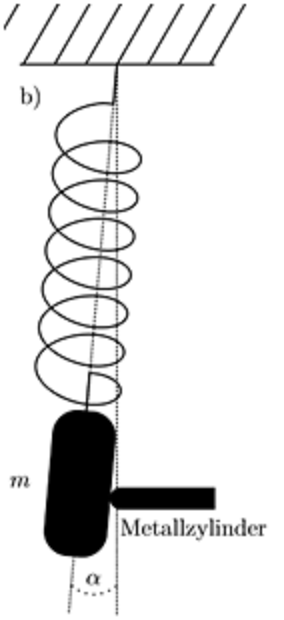
\includegraphics[width=0.2\textwidth]{Graphik/Versuch}
                \label{1}
                \caption{Versuchsskizze$^{\cite{A}}$}
\end{figure}
\noindent
Den Gleitreibungskoeffizienten $\mu$ von Stahl auf Stahl bestimmt man mittels Videoanalyse. Hinter das 400\,g Gewicht wird ein Metallzylinder so 
ausgerichtet, dass er das Gewicht berührt, wie in Abbildung (1) dargestellt. Der Metallzylinder wird zunächst so eingestellt, dass der Winkel $\alpha$ klein ist. Die Kamera wird vor dem 
Gewicht befestigt. Es wird ein Video von dem Schwingungsvorgang mit Dämpfung aufgezeichnet und, analog zu dem Vorgehen in 3.4, mit measure Dynamics 
ausgewertet. Die Aufzeichnung und Auswertung wiederholt man für einen größeren Winkel $\alpha$.

\noindent
\newpage


\section{Formeln}

\subsection{Formel für die Federkraft}
\begin{equation}
F=D \cdot x_1
\label{D}
\end{equation}

$F$ [N]: Federkraft;
$D$ [$\frac{N}{m}$] Federkonstante;
$x_1$ [m]: Längendifferenz der Feder

\subsection{Formel für die Periodendauer }

\begin{equation}
T=\sqrt{\frac{m+\frac{m_F}{3}}{D}}\cdot 2\cdot \pi
\label{T}
\end{equation}

$T$ [s]: Periodendauer;
$m$ [kg]: Angehängte Masse an die Feder;
$m_F$ [kg]: Masse der Feder

\subsection{Formel für Reibungskraft}

\begin{equation}
F_R=\mu \cdot F_N = \mu \cdot \frac{a}{h} \cdot F_G= \frac{D\cdot x_2}{2}
\end{equation}

	$F_R$ [N]: Reibkraft;
	$x_2$ [m]: Amplitudendifferenz zwischen zwei benachbarten Extrema;
	$\mu$: Gleitreibungskoeffizient;
	$F_N $ [N]: Normalkraft;
	$F_G$ [N]: Gewichtskraft;
	$h$ [m]: Ankathete zum Winkel $\alpha$;
	$a$ [m]: Gegenkathete zum Winkel $\alpha$;
	$g$: Erdbeschleunigung $g\approx 9,81\,\frac{\text{m}}{{\text{s}^2}}$
\par 
Umformen der Gleichungen für Reibung ergibt:
\begin{equation}
\mu=\frac{D \cdot x }{2 \cdot g \cdot m \cdot \cos(\alpha)}
\label{mu}
\end{equation}

\newpage

\section{ Messwerte}
\begin{figure}[H]
\centering
\caption{Messwerte weiche Feder}
\begin{tabular}{|c|c|} \hline
Masse $m$ [kg]&	Länge $l$ [m]\\ \hline
0,05	&0,27\\ \hline
0,10	&0,29\\ \hline
0,15&	0,31\\ \hline
0,20	&0,33\\ \hline
0,25&	0,35\\ \hline
0,30&	0,37\\ \hline
0,35	&0,39\\ \hline
0,40	&0,42\\ \hline
0,45	&0,43\\ \hline
\end{tabular}				
\begin{tabular}{|c|c|c|c|c|} \hline						
Masse $m$ [kg]& Zeit $t_1$ [s]& Zeit $t_2$ [s]&Zeit $t_3$ [s]\\ \hline
0,05	&3,50	&3,63	&3,59\\ \hline
0,10	&4,59	&4,68	&4,72\\ \hline
0,15	&5,35	&5,35	&5,47\\ \hline
0,20	&6,16	&6,18	&6,16\\ \hline
0,25	&6,94	&6,82	&6,78\\ \hline
0,30	&7,41	&7,34	&7,37\\ \hline
0,35 &8,09	&7,87	&8,00\\ \hline
0,40 &8,50	&8,59	&8,53\\ \hline
0,45	&9,00	&8,97	&9,03\\ \hline
\end{tabular} 
\end{figure}
\begin{figure}[H]
\centering
\caption{Messwerte harte Feder}
\begin{tabular}{|c|c|} \hline
Masse $m$ [kg]&	Länge $l$ [m]\\ \hline
0,10&	0,215\\ \hline
0,20&	0,230\\ \hline
0,30&	0,235\\ \hline
0,40&	0,245\\ \hline
0,50&	0,255\\ \hline
0,60&	0,265\\ \hline
0,70&	0,275\\ \hline
0,80&	0,285\\ \hline
0,90&	0,295\\ \hline
1,00&	0,305\\ \hline
\end{tabular}
\begin{tabular}{|c|c|c|c|c|} \hline
Masse $m$ [kg]& Zeit $t_1$ [s]& Zeit $t_2$ [s]&Zeit $t_3$ [s]\\ \hline
0,40	&4,16	&4,32	&3,97\\ \hline
0,50	&4,35	&4,32	&4,41\\ \hline
0,60	&4,68	&4,75	&4,72\\ \hline
0,70	&5,09	&5,09	&5,06\\ \hline
0,80	&5,37	&5,32	&5,47\\ \hline
0,90	&5,75	&5,72	&5,75\\ \hline
1,00	&6,00	&6,02	&6,09\\ \hline
\end{tabular}\\ 
\end{figure}
\begin{figure}[H]
\caption{Messwerte Gummi}
\centering
\begin{tabular}{|c|c|c|} \hline
Masse $m$ [kg]&	$\text{l}_\text{vor}$ [m]&	$\text{l}_\text{nach}$ [m] \\ \hline
0,05	&0,110		&0,121 \\ \hline
0,10	&0,120	&0,124 \\ \hline
0,15	&0,125	&0,127 \\ \hline
0,20	&0,127	&0,131 \\ \hline
0,25	&0,132	&0,134 \\ \hline
0,30	&0,136	&0,137 \\ \hline
0,35	&0,140	&0,140 \\ \hline
0,40	&0,144	&0,146 \\ \hline
0,45	&0,148	&0,148 \\ \hline
\end{tabular} \\
\end{figure}

\newpage

\section{ Auswertung}

\subsection{Federkonstante durch statische Methode}

Für die Bestimmung der Federkonstante in der statischen Methode benötigen wir folgende Äquivalenz:
\begin{align*}
F_G =m\cdot g = F_D = D\cdot l 
\end{align*}
Die Gewichtskraft $F_G$ können wir berechnen, was hier Beispielweise an der Masse $m=0,05$\;kg für die weiche Feder.
\begin{align*}
F_G= 0,05\,\text{kg} \cdot 9,81\,\frac{\text{m}}{\text{s}^2} = 0,49\,\frac{\text{m}\cdot \text{kg}}{\text{s}^2} = 0,49\,\text{N}
\end{align*}
Alle weiteren errechneten werte werden für beide Feder sind in nachfolgender Tabelle nachlesbar: \par
\begin{figure}[H]
\centering
\begin{minipage}{0.45\textwidth}
\vspace{-26pt}
\centering
\caption{Messwerte weiche Feder}
\begin{tabular}{|c|c|c|} \hline
Masse $m$ [kg] & Federkraft $F_D$ [N] \\ \hline
0,05	&0,49 \\ \hline
0,10	&0,98 \\ \hline
0,15	&1,47 \\ \hline
0,20	&1,96 \\ \hline
0,25	&2,45 \\ \hline
0,30	&2,94 \\ \hline
0,35	&3,43 \\ \hline
0,40	&3,92 \\ \hline
0,45	&4,41 \\ \hline
\end{tabular}				\\
\end{minipage}
\begin{minipage}{0.5\textwidth}
\vspace{-12pt}
\centering
\caption{Messwerte harte Feder}
\begin{tabular}{|c|c|c|} \hline
Masse $m$ [kg]& Federkraft $F_D$ [N] \\ \hline
0,10&	0,98 \\ \hline
0,20&	1,96 \\ \hline
0,30&	2,94 \\ \hline
0,40&	3,92 \\ \hline
0,50&	4,91 \\ \hline
0,60&	5,89 \\ \hline
0,70&	6,87 \\ \hline
0,80&	7,85 \\ \hline
0,90&	8,83 \\ \hline
1,00& 9,81 \\ \hline
\end{tabular}\\
\end{minipage}
\end{figure} 
\newpage
Daraus lässt sich ein Kraft-Länge-Diagramm erstellen, welches wie folgt aussieht:
\begin{figure}[H]
\centering
\vspace{-10pt}
\caption{ Kraft-Länge-Diagramm weiche Feder}
                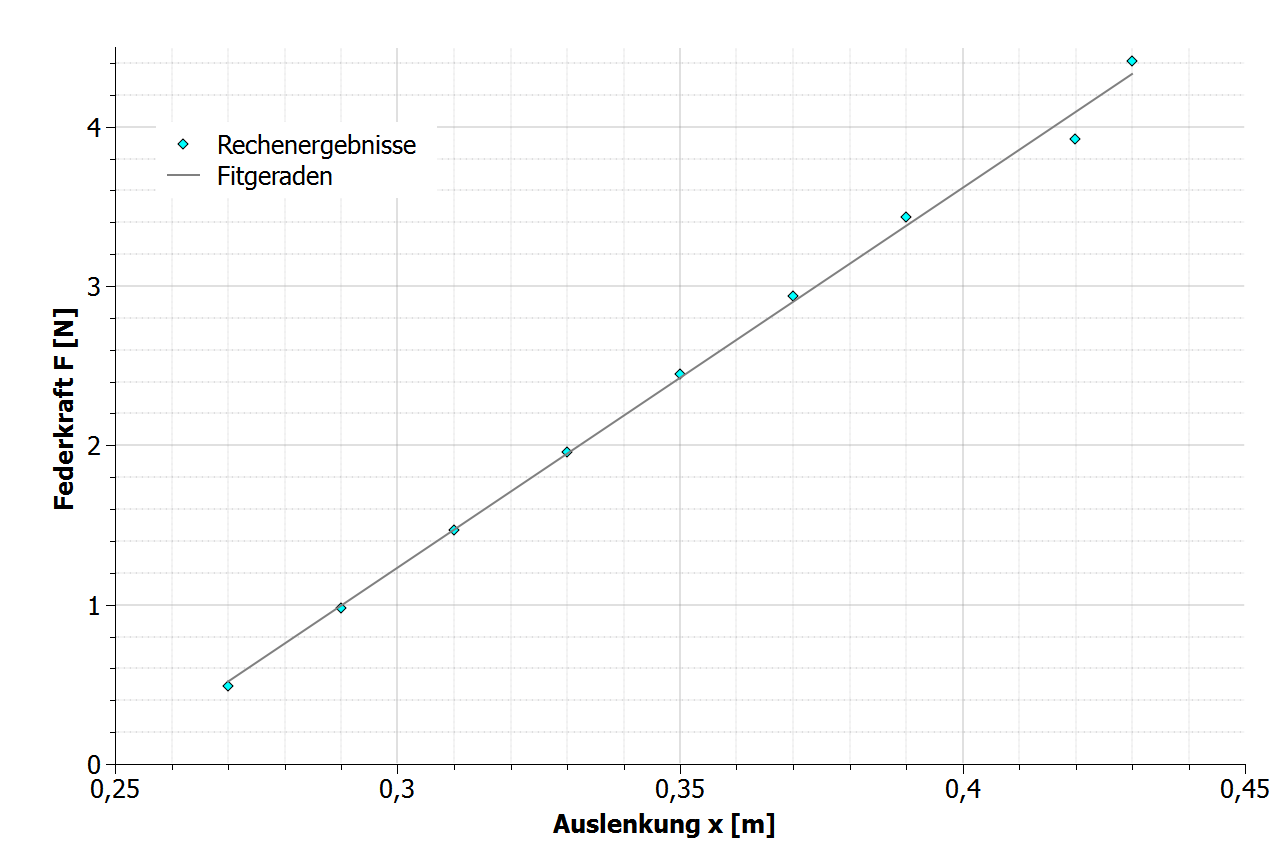
\includegraphics[width=0.7\textwidth]{Graphik/weicheFeder}
                
\caption{ Kraft-Länge-Diagramm harte Feder}
                 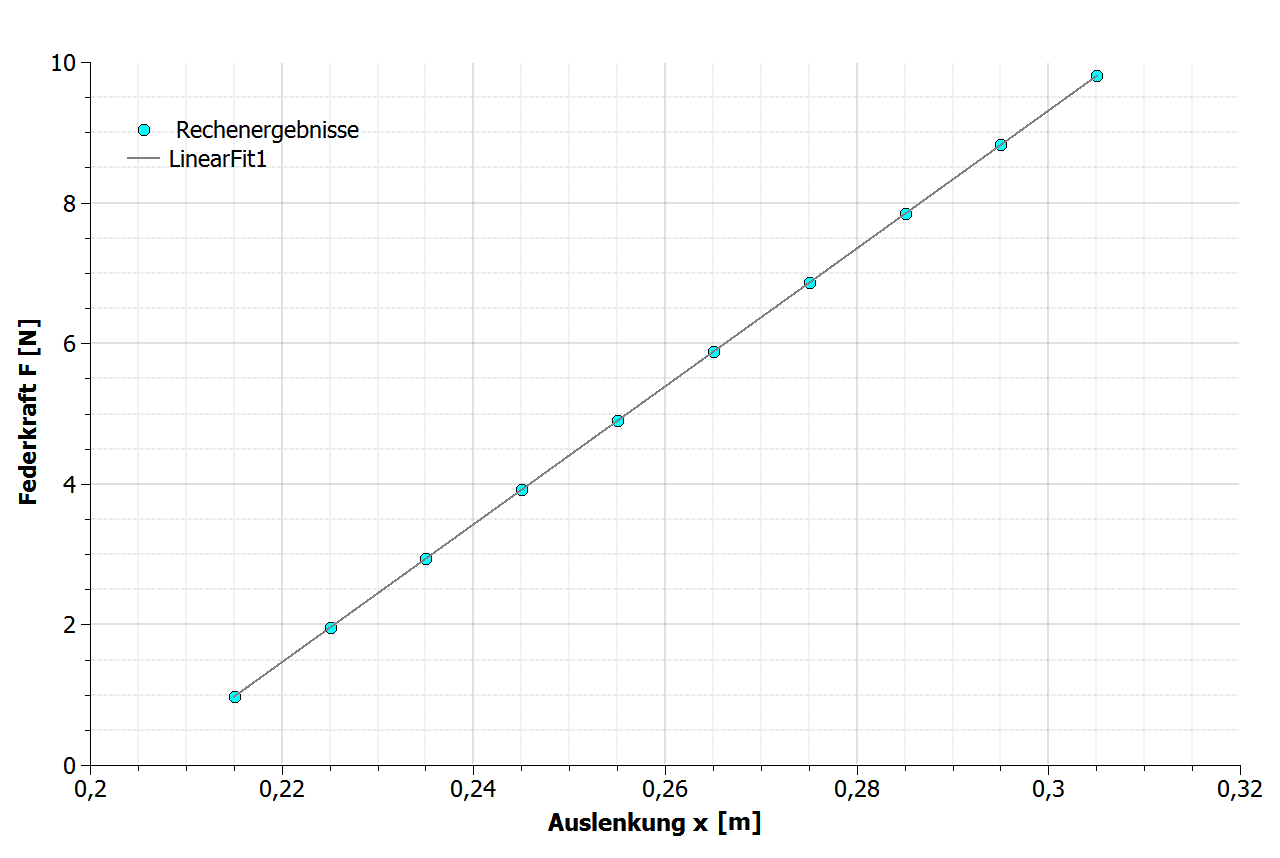
\includegraphics[width=0.7\textwidth]{Graphik/harteFeder}
\end{figure}
Durch lineare Fits mit der Geradengleichung $f(x) = a\cdot x + b$ erhalten wir dann aus der Steigung $a$ unsere jeweiligen Federkonstanten:
\begin{figure}[H]
\centering
\begin{tabular}{c|c }
Art & Federkonstante $D\,[\frac{\text{N}}{\text{m}}]$\\ \hline
weiche Feder & 23,83\\
harte Feder & 98,1\\
\end{tabular}\\
\end{figure} 
\newpage

\subsection{Federkonstante durch dynamische Methode}

Hierfür benötigen wir zuerst die Periodendauer des ungedämpften harmonischen Pendels. Durch mitteln unserer Zeitmessungen erhalten wir die Periodendauer über 10 Perioden. Wir erhalten also die Gleichung:
\begin{align*}
\bar{T}= \frac{\sum\limits^3_{k=1} t_k}{3 \cdot 10}
\end{align*}
Beispielhaft wird hier an der weichen Feder bei $m=0,05$\,kg die Periodendauer berechnet:
\begin{align*}
\bar{T}= \frac{\sum\limits^3_{k=1} t_k}{3 \cdot 10} =\frac{ t_1+t_2+t_3}{30} =\frac{ 3,50\,\text{s}+3,63\,\text{s}+3,59\,\text{s}}{30}=0,36\,\text{s}
\end{align*}
Die restlichen Werte sind in der nachfolgenden Tabelle ablesbar:
\begin{figure}[H]
\centering
\begin{minipage}{0.45\textwidth}
\centering
\caption{Messwerte weiche Feder}
\begin{tabular}{|c|c|} \hline						
\rule{0pt}{12pt} Masse $m$ [kg]& Periodendauer $\bar{T}$  [s] \\ \hline
0,05	&0,36\\ \hline
0,10	&0,47\\ \hline
0,15	&0,54\\ \hline
0,20	&0,62\\ \hline
0,25	&0,68\\ \hline
0,30	&0,74\\ \hline
0,35	&0,80\\ \hline
0,40	&0,85\\ \hline
0,45	&0,90\\ \hline
\end{tabular} 
\end{minipage}
\begin{minipage}{0.45\textwidth}
\vspace{-28pt}
\centering
\caption{Messwerte harte Feder}
\begin{tabular}{|c|c|c|c|c|} \hline
\rule{0pt}{12pt} Masse $m$ [kg]& Periodendauer $\bar{T}$ [s]\\ \hline
0,40	&0,42\\ \hline
0,50	&0,44\\ \hline
0,60	&0,47\\ \hline
0,70	&0,51\\ \hline
0,80	&0,54\\ \hline
0,90	&0,57\\ \hline
1,00	&0,60\\ \hline
\end{tabular}\\ 
\end{minipage}
\end{figure}
Nun können wir ein Periodendauer-Masse-Diagramm erstellen, wobei hier aber über die Periodendauer im Quadrat aufgetragen wird. Damit entsteht das lineares Verhältnis $\bar{T}^2 \propto m$. \newpage

Die Diagramme sehen wir folgt aus:
\begin{figure}[H]
\centering
\vspace{-10pt}
\caption{ Periodendauer-Länge-Diagramm weiche Feder}
                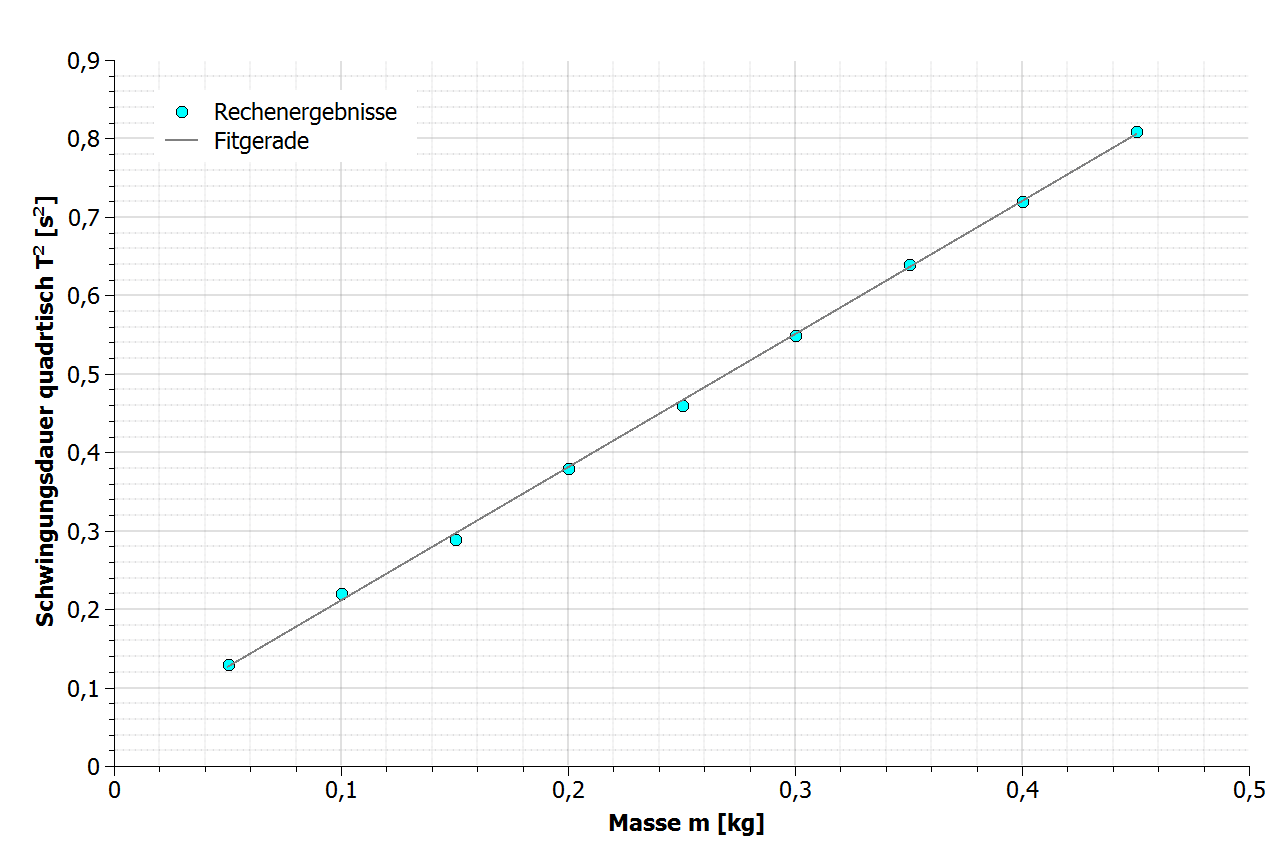
\includegraphics[width=0.7\textwidth]{Graphik/dynweichefeder}
                \label{w}
\caption{ Periodendauer-Länge-Diagramm harte Feder}
                 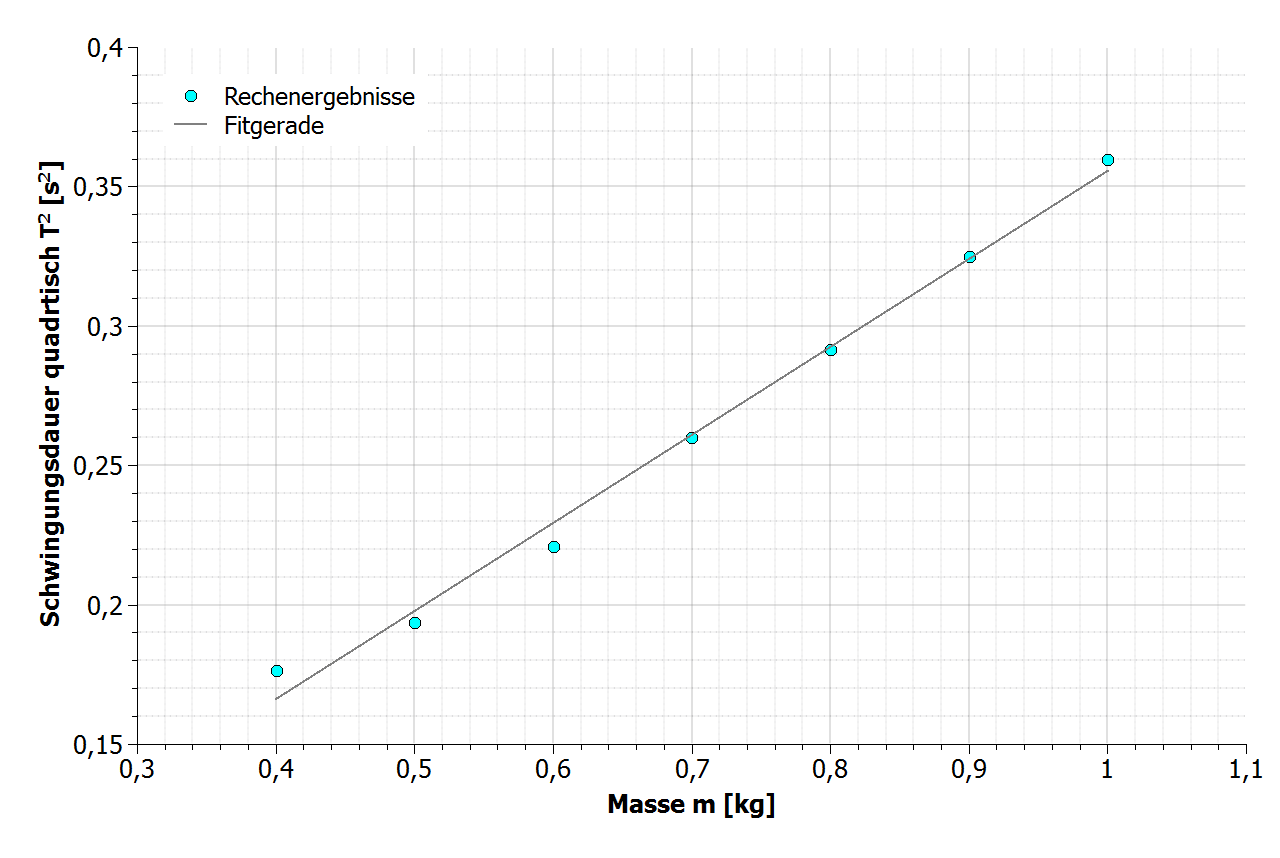
\includegraphics[width=0.7\textwidth]{Graphik/dynhartefeder}
                 \label{h}
\end{figure}
Wir können wieder einen linearen fit $f(x) =a \cdot x + b$ in unsere Diagramme einfügen. Aus diesen Erhalten wir dann für die Steigungen $a$:
\begin{figure}[H]
\centering
\begin{tabular}{c|c }
Art & Steigung $a [\,\frac{\text{s}^2}{\text{kg}}]$ \\ \hline
weiche Feder & 1,70\\
harte Feder & 0,32\\
\end{tabular}\\
\end{figure} 

\newpage

Für die Steigung ergibt sich nun aber folgendes Verhältnis:
\begin{align*}
a= \frac{4 \pi^2}{D}\qquad \Longrightarrow \qquad D_1=\frac{4 \pi^2}{a}&=\frac{4 \pi^2}{1,70\,\frac{\text{s}^2}{\text{kg}}}=23,20\,\frac{\text{N}}{\text{m}}\\
D_2=\frac{4 \pi^2}{a}&=\frac{4 \pi^2}{0,32\,\frac{\text{s}^2}{\text{kg}}}=123,25\,\frac{\text{N}}{\text{m}}
\end{align*}
und wir erhalten folgende Federkonstanten:
\begin{figure}[H]
\centering
\begin{tabular}{c|c }
Art &Federkonstante $D\,[\frac{\text{N}}{\text{m}}]$ \\ \hline
weiche Feder & 23,20\\
harte Feder & 123,25\\
\end{tabular}\\
\end{figure} 

Auf diese Werte wird im nächsten Abschnitt genauer eingegangen.

	\subsection{Berechnung Massen der Federn}

Bei den linearen Fits von den Graphiken (\ref{w}) und (\ref{h}) haben wir ein Absolutglied $b$. Zur Berechnung der Masse der Feder benötigen wir genau dieses:
\begin{figure}[H]
\centering
\begin{tabular}{c|c }
Art & Absolutglied $b$ \\ \hline
weiche Feder & 0,0400\\
harte Feder & 0,0425\\
\end{tabular}\\
\end{figure} 
Es gilt nun folgende Relation:
\begin{align*}
a\cdot x +b = \bar{T}^2 &= \frac{4 \pi^2}{D} (m+m_F) \\
~\\
\overset{a\cdot x = \frac{4 \pi^2}{D} m}{\Longrightarrow} \qquad b&= \frac{4 \pi^2}{D} m_F\\
\Longrightarrow \qquad  m_F&= \frac{D}{4 \pi^2} b
\end{align*}
und wir erhalten folgende Massen für unsere Federn:	
\begin{figure}[H]
\centering
\begin{tabular}{c|c|c }
Art & Masse Feder $m_F$ [kg]  &  gemessene Masse Feder $m_F$ [kg]\\ \hline
weiche Feder & 0,024 & 0,062\\
harte Feder & 0,133 & 0,038\\
\end{tabular}\\
\end{figure} 
Bei unseren Rechnungen erhalten wir für unsere weiche Feder etwa identische Ergebnisse.  Doch bei der harten Feder erhalten wir relativ starke 
Abweichungen, vor allem bei der Masse der Feder mit einem Faktor von $\approx 10$. Dies kann zum einen eventuell daran liegen, dass wir die Masse der 
Feder homogen verteilt annehmen, oder, eher unwahrscheinlich, dass die Feder mal in vorherigen Versuchen überspannt wurde.	\par

Als Alternative gibt  es nun folgende Möglichkeit. Statt wie vorher die Masse $m=0$ zu setzen, setzen wir diesmal $T=0$. Damit erhalten wir folgende Gleichung:
\begin{align*}
0=\frac{4\pi^2}{D}\cdot (m+m_F)=\frac{4\pi^2}{D}\cdot (m)+b = \frac{4\pi^2}{D}\cdot (m)+0,0425
\end{align*}
Hierraus ergibt sich dann, dass $m$ die Masse der Feder sein muss. Es ergibt sich sich hier für $\l m\r = 0,133$\,Kg. Ein etwas besseres Ergebnis, dennoch sehr weit daneben.

\subsection{Elastizitätsverhalten von Gummi}

Für diesen Versuch mussten wir lediglich unsere gemessenen Wert in ein Ausdehnung-Masse-Diagramm:
\begin{figure}[H]
\centering
\caption{Masse-Auslenkung-Diagramm}
                \includegraphics[width=0.75\textwidth]{Graphik/gummi}
\end{figure}
\newpage
Bei Betrachtung der Länge von Gummi, fällt auf, dass bei der 2.Messung mit abnehmen der Gewichte, das Gummi nicht mehr die Ausgangslänge erreicht. Das 
war zu erwarten. Ab 150 Gramm sieht man bei der ersten Messung, die Elastizität des Gummis nicht mehr gegeben ist wir als über die Elastizitätsgrenze des Gummi gekommen sind. 
Ab dieser Grenze tritt ein irreversible plastische Verformung, d.h. das Gummi verhält sich nicht mehr elastisch.


\subsection{Federkonstante über harmonische Schwingung}

In diesem Teil des Versuch erhielten wir im Versuch folgendes Diagramm:
\begin{figure}[H]
\centering
\caption{Masse-Auslenkung-Diagramm}
                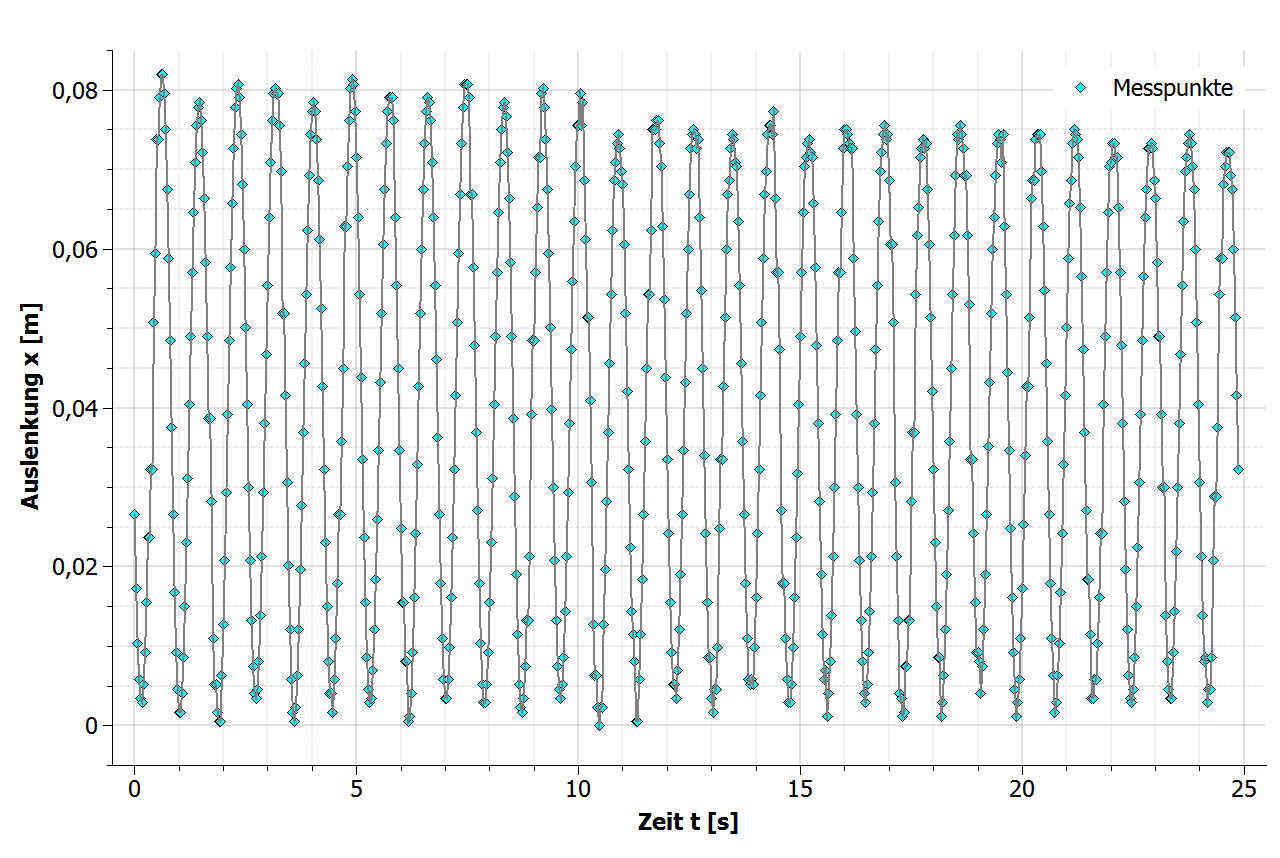
\includegraphics[width=\textwidth]{Graphik/Federkonstante}
\end{figure}
Nun haben wir vom ersten Hochpunkt bis zum letzten Hochpunkt die Zeiten ermittelt und damit die Periodendauer errechnet. Wir haben von 0,6333\,s bis 24,6333\,s 29 Hochpunkte und erhalten damit folgende Schwingungsdauer:
\begin{align*}
T=\frac{(24,6333-0,6333)}{28}=0,86\,\text{s}
\end{align*}
Sie stimmt damit unserer Messung der dynamischen Methode überein, wo wir bei 400 Gramm eine Periodendauer von $0,85$\,s hatten.\par

Nun können wir mit der Formel
\begin{align*}
T^2 = \frac{4\pi^2 \cdot m}{D}
\end{align*}
die Federkonstante ausrechnen.
Wir erhalten in diesem Fall durch umformen:
\begin{align*}
D &= \frac{4\pi^2 \cdot m}{T^2} \\
&= \frac{4\pi^2 \cdot 0,4\,\text{kg}}{0,86^2\,\text{s}^2} \\
&=21,47\,\frac{\text{N}}{\text{m}}
\end{align*}
Welche relativ nahe an der Federkonstante in Abschnitt 6.2 liegt.

\newpage

\subsection{Berechnung des Gleitreibungskoeffizienten Stahl-Stahl}

In diesem und letzten Teil des Versuchs erhielten wir zwei Auslenkung-Zeit-Diagramme, welche wie folgt aussehen:
\begin{figure}[H]
\centering
\vspace{-10pt}
\caption{ Auslenkung-Zeit-Diagramm kleiner Winkel}
                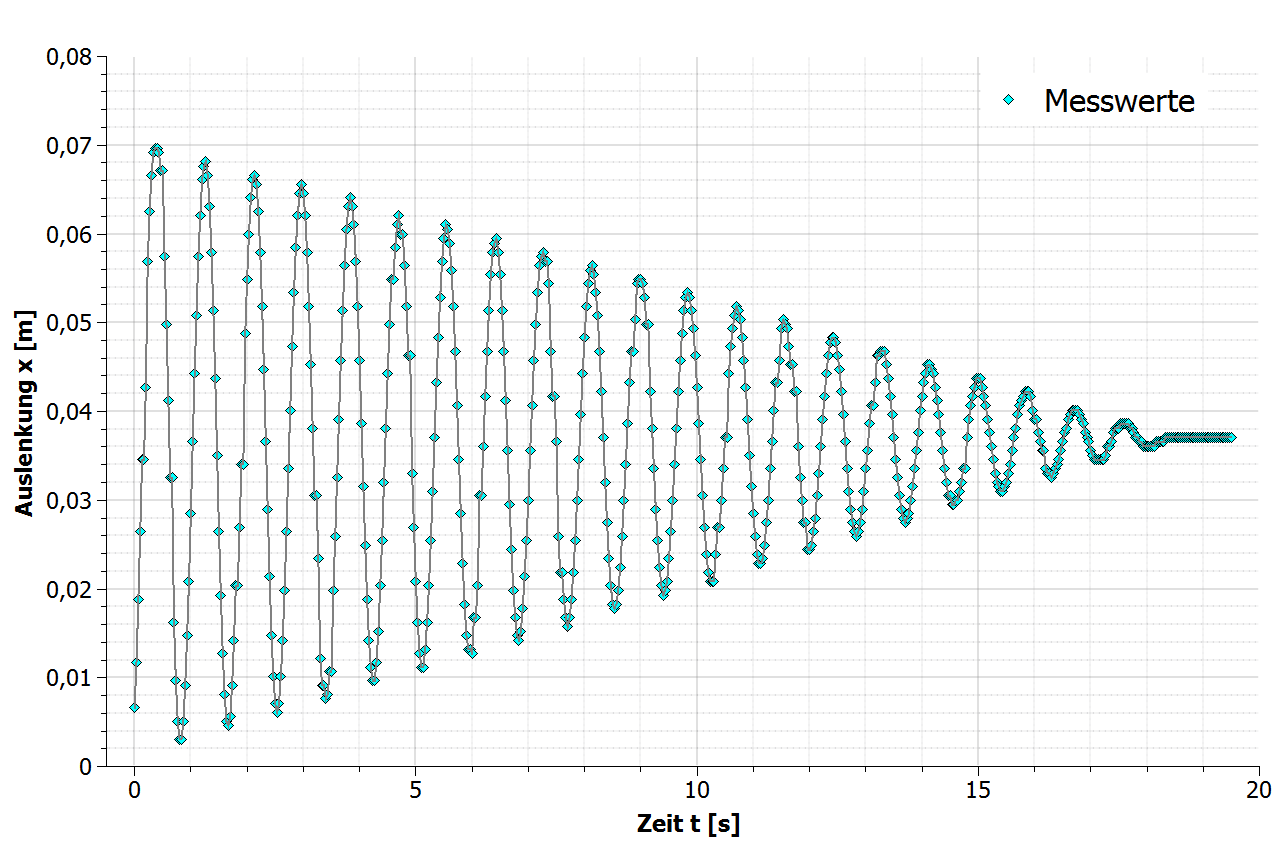
\includegraphics[width=0.7\textwidth]{Graphik/kleinerWinkel}
\caption{ Auslenkung-Zeit-Diagramm großer Winkel}
                 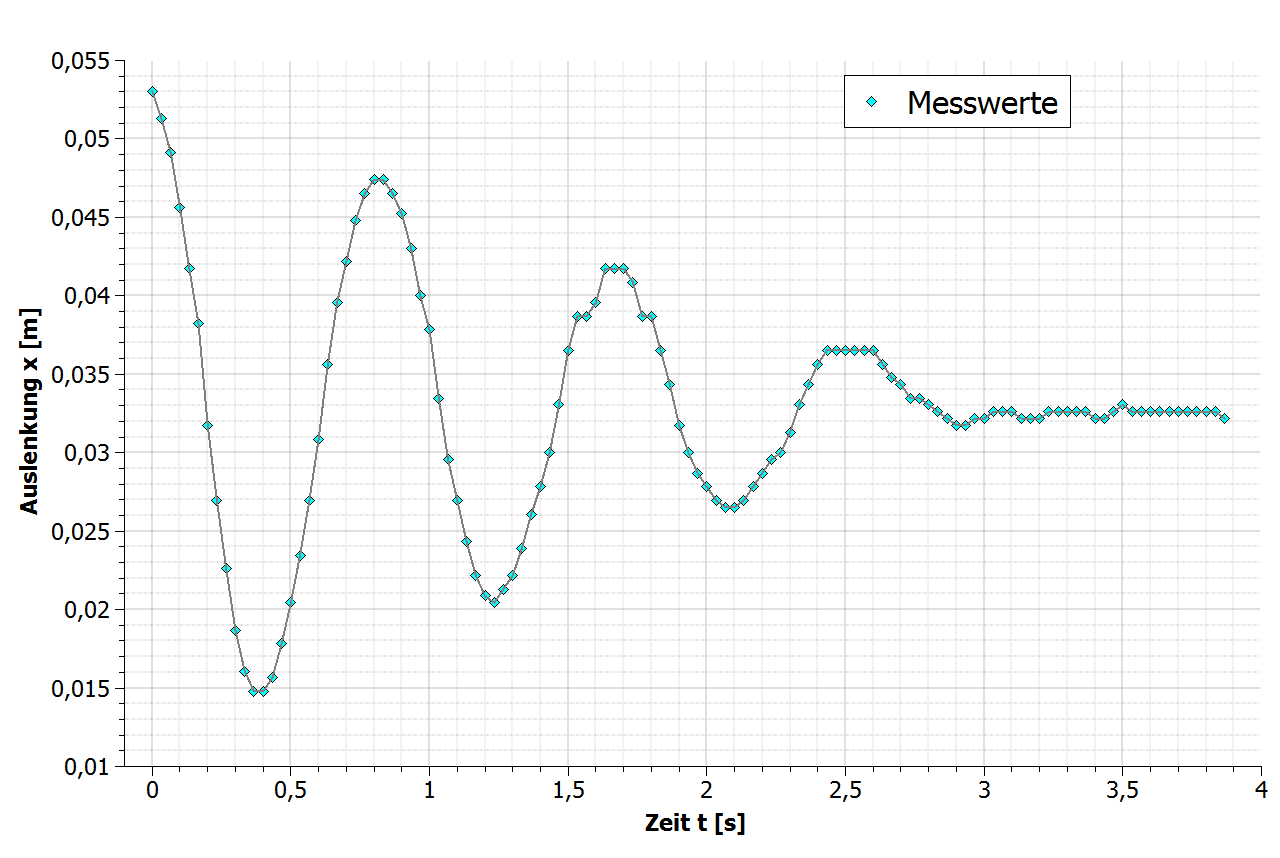
\includegraphics[width=0.7\textwidth]{Graphik/grosserWinkel}
\end{figure}
Um nun mit der Formel (\ref{mu}) nun den Gleitreibungskoeffizienten zu berechnen, benötigen wir nun den Winkel $\alpha$.\par

In dem nachfolgenden Bild wird skizzenhaft das Dreieck dargestellt, welches für für die Berechnung von $\alpha$ brauchen:
\begin{figure}[H]
\centering
\vspace{-10pt}
                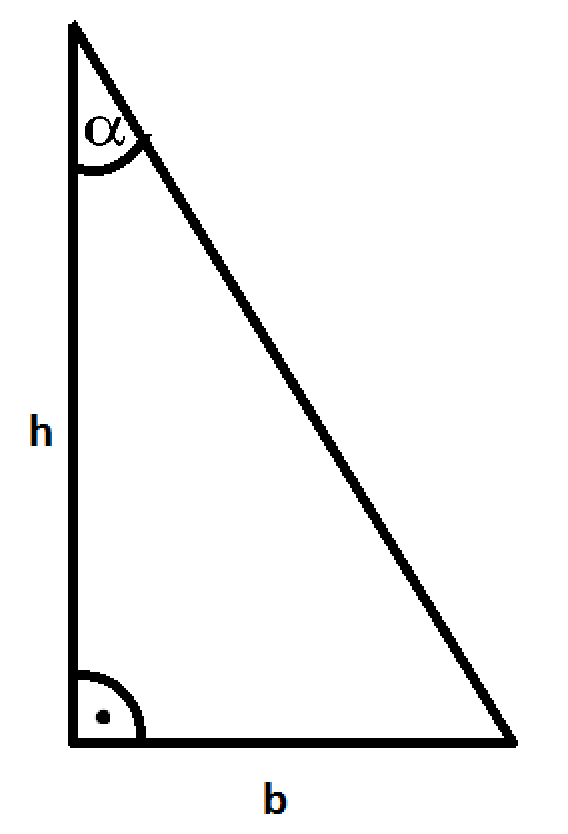
\includegraphics[width=0.2\textwidth]{Graphik/Dreieck}
\end{figure}
wir haben folgende Werte, wobei $\alpha = \arctan(\frac{b}{h})$ ist und damit
\begin{align*}
\alpha_1 &= \arctan(\frac{6\,\text{cm}}{50\,\text{cm}})=6,84^{\circ}\\
\alpha_2 &= \arctan(\frac{8\,\text{cm}}{50\,\text{cm}})=9,09^{\circ}
\end{align*}
somit haben wir:
\begin{figure}[H]
\centering
\begin{tabular}{c|c|c }
Breite $b$ [cm] & Höhe $h$ [cm]  & Winkel $\alpha$  [$^{\circ}$]\\ \hline
6 & 50 & 6,84\\
8 & 50 & 9,09\\
\end{tabular}\\
\end{figure} 
Zudem benötigen wir $x$. Hierbei ist $x$ Der Abstand von eine Hochpunkt zum nächsten Tiefpunkt.
Somit können wir Gleitreibungskoeffizienten von Stahl-Stahl ausrechnen:
\begin{align*}
\mu_1&=\frac{D \cdot x }{2 \cdot g \cdot m \cdot \cos(\alpha)}=\frac{21,47\,\frac{\text{N}}{\text{m}} \cdot (4,7399-1,473)\,\text{m} }{100 \cdot 2 \cdot 9,81\,\frac{\text{m}}{{\text{s}^2}} \cdot 0,4\,\text{kg} \cdot \cos(6,84^{\circ})} =0,09\\
\mu_2&=\frac{D \cdot x }{2 \cdot g \cdot m \cdot \cos(\alpha)}=\frac{21,47\,\frac{\text{N}}{\text{m}} \cdot  (6,9661-0,3051)\,\text{m} }{100 \cdot 2 \cdot 9,81\,\frac{\text{m}}{{\text{s}^2}} \cdot 0,4\,\text{kg} \cdot \cos(9,09^{\circ})} =0,18
\\
\end{align*}
und damit erhalten wir folgendes Ergebnis:
\begin{figure}[H]
\centering
\begin{tabular}{c|c|c|c|c }
Breite $b$ [cm] & Höhe $h$ [cm]  & Winkel $\alpha$  [$^{\circ}$] & Gleitreibungskoeffizient $\mu$ & Literaturwert$^{\cite{1}}$\\ \hline
6 & 50 & 6,84 &	 0,09	& 	0,1 \\
8 & 50 & 9,09 & 0,18		&		0,17\\
\end{tabular}\\
\end{figure} 
Die ausgerechneten Werte haben relativ kleine Abweichungen zu den Literaturwerten.
\newpage


\section{Fehlerrechnung}

Für diesen Versuch soll eine Fehlerfortpflanzung der Federkonstante sowohl in der statischen als auch in der dynamischen Methode und dann eine Fehlerfortpflanzung für den Gleitreibungskoeffizienten. Vorerst können folgend Werte angenommen werden
\begin{center}
$\Delta m =0,1\,\text{g}=1\cdot 10^{-4}\,\text{kg}$ \par
$\Delta x =0,1\,\text{cm}=1\cdot 10^{-3}\,\text{m}$ \par
$\Delta \alpha =0,1\,^{\circ}$
$\Delta t = 0,5\,\text{s}$
\end{center}
Es werden erst Beispielrechnungen bei der weichen Feder durchgeführt und dann zum Schluss eine Tabelle mit allen errechneten Fehler für beide Federn mit Originalwert angegeben.

\subsection{Fehlerrechnung der statischen Methode}

Es gilt für die Statische Methode folgende Fehlerfortpflanzung für $\Delta D$. Wir verwenden hier die Messwerte für die Messung bei 150\,g. Da dort der Messpunkt exakt auf der Fitgeraden liegt:
\begin{align*}
\Delta D &=\l \frac{\partial D}{\partial x} \cdot \Delta x \r +\l \frac{\partial D}{\partial m} \cdot \Delta m \r = \l  \frac{-F_R}{x^2} \r  \cdot \Delta x+ \l \frac{g}{x} \r\cdot \Delta m\\
&= \l  \frac{-1,47\,\text{N}}{0,31^2\,\text{m}^2} \r  \cdot 1\cdot 10^{-3}\,\text{m}+ \l \frac{9,81\,\frac{\text{m}}{{\text{s}^2}}}{0,31\,\text{m}} \r\cdot 1\cdot 10^{-4}\,\text{kg}=0,18\,\frac{\text{N}}{\text{m}}
\end{align*}

\subsection{Fehlerrechnung dynamische Methode}

Den ersten Fehler haben wir in der Periodendauer. Der Fehler ergibt sich recht schnell durch:	
\begin{align*}
\Delta\bar{T}&=\frac{\partial \frac{\sum\limits^3_{k=1} t_k}{3 \cdot 10}}{\partial t_k} \cdot \Delta t =\frac{\sum\limits^3_{k=1} \Delta t}{3 \cdot 10}\\
~\\
&=\frac{3\cdot \Delta t}{3 \cdot 10} = \frac{\Delta t}{10} = \frac{0,5\,\text{s}}{10} = 0,05\,\text{s}
\end{align*}
Hier wird ersichtlich, dass durch mehrere Messungen unsere Fehler nicht kleiner werden, jedoch durch mitnehmen von mehr Perioden.
\newpage
Damit erhalten wir für die Federkonstante folgende Fehlerfortpflanzung für die Messung bei 400\,G:
\begin{align*}
\Delta D&=\l \frac{\partial D}{\partial m}\r\cdot \Delta m + \l \frac{\partial D}{\partial \bar{T}}\r\cdot \Delta \bar{T} \\
~\\
&=\l\frac{4 \cdot \pi ^2}{T^2} \r \cdot \Delta m +  \l \frac{-8 \cdot \pi ^2 \cdot m}{T^3}\r\cdot \Delta \bar{T} \\
~\\
&=\l\frac{4 \cdot \pi ^2}{0,85^2\text{s}^2} \r \cdot 1\cdot 10^{-4}\,\text{kg} +  \l \frac{-8 \cdot \pi ^2 \cdot 0,4\,\text{kg}}{0,85^3\text{s}^3}\r\cdot  0,05\,\text{s}=2,58\,\frac{\text{N}}{\text{m}}
\end{align*}

\subsection{Fehlerrechnung  Gleitreibungskoeffizienten}
Mit Hilfe des Abschnitts Fehlerrechnung dynamische Methode erhalten wir für $\Delta \mu$:
\begin{align*}
\Delta \mu &=\l \frac{\partial  \mu}{\partial D}\cdot \Delta D \r +  \l \frac{\partial  \mu}{\partial m}\cdot \Delta m \r+  \l \frac{\partial  \mu}{\partial \alpha}\cdot \Delta \alpha \r \\
~\\
\Delta \mu&= \l \frac{x }{2 \cdot g \cdot m \cdot \cos(\alpha)}\cdot \Delta D \r +  \l \frac{-D \cdot x }{2 \cdot g \cdot m^2 \cdot \cos(\alpha)} \cdot \Delta m \r+  \l \frac{-D \cdot x \cdot sin(\alpha)}{2 \cdot g \cdot m \cdot \cos^2(\alpha)}\cdot \Delta \alpha \r \\
~\\
\Delta \mu &= \l \frac{3,27\cdot 10^{-2}\text{m} }{2 \cdot 9,81\,\frac{\text{m}}{{\text{s}^2}} \cdot 0,4\,\text{kg} \cdot 0,99}\cdot 2,58\,\frac{\text{N}}{\text{m}} \r +  \l \frac{21,47\,\frac{\text{N}}{\text{m}}  \cdot 3,27\cdot 10^{-2}\text{m} }{2 \cdot 9,81\,\frac{\text{m}}{{\text{s}^2}} \cdot (0,4\,\text{kg})^2 \cdot 0,99} \cdot 1\cdot 10^{-4}\,\text{kg} \r \\
&+  \l \frac{21,47\,\frac{\text{N}}{\text{m}} \cdot 3,27\cdot 10^{-2}\text{m} \cdot 0,12}{2 \cdot 9,81\,\frac{\text{m}}{{\text{s}^2}} \cdot 0,4\,\text{kg} \cdot 0,99^2}\cdot 0,1\r \\
~\\
\Delta \mu &= 0,011 + 2,26\cdot 10^{-5} + 1,1\cdot10^{-3}\\
~\\
\Delta \mu &= 0,012
\end{align*}
\newpage
Zusammen erhalten wir folgende Werte:
\begin{figure}[H]
\centering
\begin{tabular}{l|c|c}
Fehler & weiche Feder & harte Feder \\ \hline
\rule{0pt}{12pt} $\Delta D_{\text{statisch}}$ & $0,18\,\frac{\text{N}}{\text{m}}$ & $0,11\,\frac{\text{N}}{\text{m}}$\\
\rule{0pt}{12pt}  $\Delta \bar{T}$ & $0,5\,\text{s}$ & $0,5\,\text{s}$\\
\rule{0pt}{12pt}  $\Delta D_{\text{dyn}}$ & $2,58\,\frac{\text{N}}{\text{m}}$ & $19,20\,\frac{\text{N}}{\text{m}}$
\rule{0pt}{12pt} 
\end{tabular}\\
\end{figure} \par
\begin{figure}[H]
\centering
\begin{tabular}{l|c|c}
Fehler & kleiner Winkel & großer Winkel \\ \hline
\rule{0pt}{12pt} $\Delta \mu$ &0,012 & 0,028\\
\end{tabular}\\
\end{figure} 

\section{Zusammenfassung}


Ziel des Versuchs war zunächst die Bestimmung der Federkonstanten D mithilfe der statischen und der dynamischen Methode. 
Für uns ergaben sich folgende Werte bei der Bestimmung der Federkonstanten:
\begin{figure}[H]
\centering
\begin{tabular}{l|c|c }
\rule{0pt}{12pt}Art & $D_{\text{stat}}\,[\frac{\text{N}}{\text{m}}]$& $D_{\text{stat}}\,[\frac{\text{N}}{\text{m}}]$\\ \hline
\rule{0pt}{12pt}weiche Feder & 23,83$\pm$0,18&	23,20$\pm$2,58 	\\
\rule{0pt}{12pt}harte Feder & 98,1$\pm$0,11&	123,25$\pm$19,20 \\
\end{tabular}\\
\end{figure} 
Wir sehen, dass bei der weichen Feder die beiden Methoden nahezu identisch sind. Bei der harten Feder entstehen jedoch große Abweichungen, die wir uns nicht wirklich erklären können. 
Ein weiteres Ziel war es die Masse der Federn zu errechnen. Wir erhielten
\begin{figure}[H]
\centering
\begin{tabular}{c|c|c }
Art & Masse Feder $m_F$ [kg]  &  gemessene Masse Feder $m_F$ [kg]\\ \hline
weiche Feder & 0,077 & 0,062\\
harte Feder & 0,380 & 0,038\\
\end{tabular}\\
\end{figure} 
Auch hier haben wir bei der weichen Feder nahezu identische Ergebnisse, prozentual haben wir bei der weichen Feder aber eine Abweichung von 19,5\%.
Bei der harten haben wir eine sehr große Abweichung. Eine andere alternative Berechnung ergab bei uns eine Masse von 133 Gramm, immer noch eine Abweichung von 71,43\%. Erklären können wir uns dies nur dadurch, dass wir die Massenverteilung der Federn homogen annehmen. Vielleicht ist dies hier nicht der Fall.
\newpage
Auch die elastischen Eigenschaften von Gummi wurden bei diesem Versuch betrachtet. Heraus kam, dass Gummi, wenn man zu es überdehnt, nicht mehr elastisch ist. Es findet ein irreversible plastische Verformung nach dieser  Elastizitätsgrenze statt, was im Grunde heißt, dass das Gummi bei Entlastung nicht mehr auf seine Originallänge zurückzieht.\par

Man kann auch über die harmonische Schwingung die Federkonstante bestimmen. In diesem Fall sollten wir die Federkonstante $D$ für die weiche Feder berechnen. Wir erhielten eine Federkonstante von 
\begin{center}
$D =21,47\,\frac{\text{N}}{\text{m}}$
\end{center}
Im Vergleich zur dynamischen Methode haben wir hier eine Abweichung von lediglich $8\%$ \par

Im letzten Teil des Versuchs sollte der Gleitreibungskoeffizient von Stahl auf Stahl ermittelt für zwei verschiedene Winkel.
Wir erhielten:
\begin{figure}[H]
\centering
\begin{tabular}{c|c}
 Gleitreibungskoeffizient $\mu$ & Literaturwert$^{\cite{1}}$\\ \hline
0,09	$\pm$ 0,012	& 	0,1 \\
0,18	$\pm$0,028&		0,17\\
\end{tabular}\\
\end{figure} 



\newpage
\section{Literaturverzeichnis}

\renewcommand{\refname}{~}
\vspace{-30pt}
\begin{thebibliography}{xx}
	\bibitem[1]{1}		\textit{ http://www.schweizer-fn.de/stoff/reibwerte/reibwerte.php}; \\
								 abgerufen am 07.07.2015
   \bibitem[2]{2}  	\textit{\glqq M20 Das Federpendel\grqq , in 	\\
   					http://www3.physik.uni-stuttgart.de/studium/praktika/ap/}, \\
   					unter \textit{http://www3.physik.uni-stuttgart.de/studium/praktika/ap/pdf\_dateien/M20.pdf}; \\
   								abgerufen am  07.07.2015

   \bibitem[A]{A}  	Graphik aus \textit{\glqq M20 Das Federpendel\grqq , in 	\\
   					http://www3.physik.uni-stuttgart.de/studium/praktika/ap/}, \\
   					unter \textit{http://www3.physik.uni-stuttgart.de/studium/praktika/ap/pdf\_dateien/M20.pdf}; \\
   								abgerufen am  07.07.2015
\end{thebibliography}

\section{Anhang}

\end{document}